% Compile using: TEXINPUTS=minted/source: pdflatex -shell-escape %
\documentclass[14pt,utf8,notheorems,compress,t]{beamer}
\usepackage{etex}

\usepackage[english]{babel}

\RequirePackage[all]{xy}
\usepackage{mathtools}
\usepackage{booktabs}
\usepackage{array}
\usepackage{ragged2e}
\usepackage{multicol}
\usepackage{tabto}
\usepackage{xstring}

\usepackage{minted}

\usepackage[protrusion=true,expansion=true]{microtype}

\setlength\parskip{\medskipamount}
\setlength\parindent{0pt}

\renewcommand{\U}{\mathcal{U}}
\renewcommand{\P}{\mathcal{P}}
\newcommand{\NN}{\mathbb{N}}
\newcommand{\id}{\mathrm{id}}
\newcommand{\ZZ}{\mathbb{Z}}
\newcommand{\QQ}{\mathbb{Q}}
\newcommand{\RR}{\mathbb{R}}
\newcommand{\Id}{\mathrm{Id}}
\newcommand{\Sh}{\mathrm{Sh}}
\newcommand{\fst}{\mathsf{fst}}
\newcommand{\snd}{\mathsf{snd}}
\newcommand{\inv}{\mathsf{inv}}
\newcommand{\refl}{\mathsf{refl}}
\newcommand{\ap}{\mathsf{ap}}
\renewcommand{\succ}{\mathsf{succ}}
\newcommand{\seg}{\mathsf{seg}}
\newcommand{\base}{\mathsf{base}}
\newcommand{\lloop}{\mathsf{loop}}
\newcommand{\ua}{\mathsf{ua}}
\newcommand{\code}{\mathsf{code}}
\newcommand{\surf}{\mathsf{surf}}
\newcommand{\merid}{\mathsf{merid}}
\newcommand{\N}{\mathsf{N}}
\renewcommand{\S}{\mathsf{S}}
\newcommand{\Cyl}{\mathrm{Cyl}}
\newcommand{\IsContr}{\mathsf{IsContr}}
\newcommand{\IsMereProp}{\mathsf{IsMereProp}}
\newcommand{\IsSet}{\mathsf{IsSet}}
\newcommand{\IsEquiv}{\mathsf{IsEquiv}}
\newcommand{\LEM}{\mathsf{LEM}}
\newcommand{\UIP}{\mathsf{UIP}}
\newcommand{\fib}{\mathsf{fib}}
\newcommand{\List}{\mathsf{List}}
\newcommand{\defeq}{\vcentcolon=}
\newcommand{\defeqv}{\vcentcolon\equiv}
\newcommand{\ct}{%
  \mathchoice{\mathbin{\raisebox{0.5ex}{$\displaystyle\centerdot$}}}%
             {\mathbin{\raisebox{0.5ex}{$\centerdot$}}}%
             {\mathbin{\raisebox{0.25ex}{$\scriptstyle\,\centerdot\,$}}}%
             {\mathbin{\raisebox{0.1ex}{$\scriptscriptstyle\,\centerdot\,$}}}
}
\renewcommand{\_}{\mathpunct{.}}
\newcommand{\fix}{\mathsf{fix}}
\newcommand{\styledhref}[2]{\href{#1}{\underline{#2}}}

\newtheorem{axiom}{Axiom}

\title{Double-negation translation and\\ CPS transformation}
\author{
  \texorpdfstring{
    \vspace{-1em} \\
    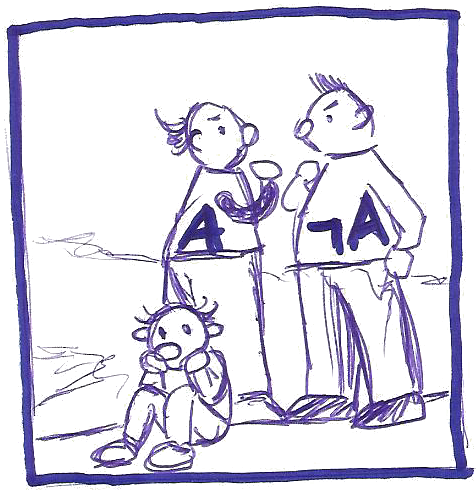
\includegraphics[scale=0.6]{lem} \\[0.5em]
    Ingo Blechschmidt \\[-0.3em]
    {\scriptsize June 3rd, 2015 at KU Leuven}%
  }{Ingo Blechschmidt}
}
\date{June 3d, 2015}

\usetheme{Warsaw}
\usecolortheme{seahorse}
%\usefonttheme{default}?
\usepackage[T1]{fontenc}
\usepackage{libertine}
\usefonttheme{serif}
%\usepackage{libertine}?
%\usepackage{mathpazo}
\useinnertheme{rectangles}


\setbeamertemplate{title page}[default][colsep=-1bp,rounded=false,shadow=false]
\setbeamertemplate{frametitle}[default][bg=red,colsep=-2bp,rounded=false,shadow=false,center]
\setbeamertemplate{blocks}[rounded][shadow=false]

\setbeamertemplate{frametitle}{%
  \vskip1em%
  \leavevmode%
  \begin{beamercolorbox}[dp=1ex,center]{}%
      \usebeamercolor[fg]{item}{\textbf{\textsf{\Large \insertframetitle}}}
  \end{beamercolorbox}%
}

\setbeamertemplate{footline}{%
  \leavevmode%
  \hfill%
  \begin{beamercolorbox}[ht=2.25ex,dp=1ex,right]{}%
    \usebeamerfont{date in head/foot}
    \insertframenumber\,/\,\inserttotalframenumber\hspace*{1ex}
  \end{beamercolorbox}%
  \vskip0pt%
}

\setbeamertemplate{headline}{}
\setbeamertemplate{navigation symbols}{}

\newcommand{\floatbox}[3]{%
  \raisebox{0pt}[0pt][0pt]{%
    \begin{picture}(0,0)(#1,#2)#3\end{picture}\leavevmode%
  }%
}

\newcommand{\backupstart}{
  \newcounter{framenumberpreappendix}
  \setcounter{framenumberpreappendix}{\value{framenumber}}
}
\newcommand{\backupend}{
  \addtocounter{framenumberpreappendix}{-\value{framenumber}}
  \addtocounter{framenumber}{\value{framenumberpreappendix}} 
}

\newcommand{\hil}[1]{{\usebeamercolor[fg]{item}{\textbf{#1}}}}

\newcommand{\img}[3]{\begin{center}\includegraphics[scale=#1]{#2}\\\scriptsize#3\end{center}}
%\newcommand{\imageslide}[3]{\frame{\frametitle{#1}\img{#2}{#3}}}

\IfSubStr{\jobname}{\detokenize{notes}}{
  \setbeameroption{show notes}
}{
  \setbeameroption{hide notes}
}
\setbeamertemplate{note page}[plain]

\newenvironment{changemargin}[2]{%
  \begin{list}{}{%
    \setlength{\topsep}{0pt}%
    \setlength{\leftmargin}{#1}%
    \setlength{\rightmargin}{#2}%
    \setlength{\listparindent}{\parindent}%
    \setlength{\itemindent}{\parindent}%
    \setlength{\parsep}{\parskip}%
  }%
  \item[]}{\end{list}}

\graphicspath{{images/}}

\begin{document}

\frame[plain,c]{
  \begin{center}
    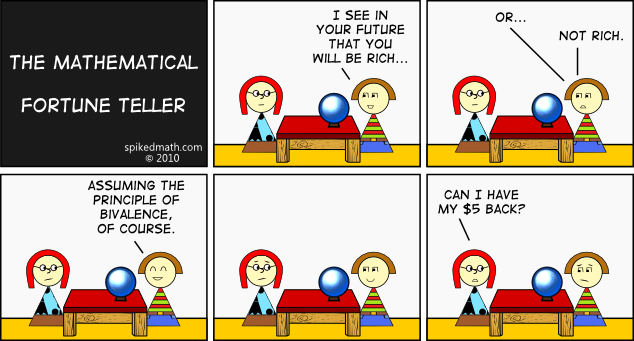
\includegraphics[scale=0.65]{fortune-teller}
  \end{center}
}

\frame{\titlepage}

\note{
  \textcolor{red}{This annotated version of the slides is not yet finished.}

  Expect references and more explanations in the next few days.
}

\note{\fontsize{8pt}{9.6}\selectfont
  \begin{center}\large\textbf{Abstract}\end{center}

  \begin{changemargin}{2.5em}{2.5em}
    \justifying
    Constructive mathematicians don't use the law of excluded middle, which
    approximately says that for any proposition~$P$, either~$P$ is true or~$\neg P$
    is true. Several advantages emerge from this rejection, for instance one
    can mechanically extract algorithms from constructive proofs of existence
    statements and rigorously work with non-standard \emph{dream axioms} which are
    plainly false in classical mathematics, such as \emph{any function is
    smooth}.

    For communicating with classicial mathematicians, constructive
    mathematicians can employ the \emph{double-negation translation}. This
    device associates to any formula a translated formula in such a way that
    a given formula holds classically if and only if its translation holds
    constructively.

    The talk will give an introduction to these topics and discuss the
    intriguing relationship of the double-negation translation with the
    well-known con\-tin\-u\-a\-tion-pas\-sing style transformation: In some sense, they are
    the same. This is a beautiful facet of \emph{computational trinitarianism}.

    For the first part of the talk, no background in formal logic or
    constructive mathematics is required. For the second part of the talk,
    one should be vaguely familiar with the continuation-passing style
    transformation.
  \end{changemargin}
}

\newcommand{\classicalcontent}{
  \begin{changemargin}{2.5em}{2.5em}
    \justifying

    By the Curry--Howard correspondence intuitionistic
    proofs have computational content. By the double-negation translation, we
    see that \emph{classical proofs too have computational content}.

    As long as we stay in the continuation monad, the required bluffing and
    cheating will not be apparent.

    Care must be taken when leaving the continuation monad (for instance by
    supplying the identity continuation), since then we might obtain
    \emph{incorrect results}.
  \end{changemargin}
}

\note{
  \begin{center}\large\textbf{Teaser}\end{center}

  \classicalcontent
}

\frame{\frametitle{Outline}\begin{itemize}\item[]\footnotesize\tableofcontents\end{itemize}}

\section{Constructive mathematics}

\subsection{The law of excluded middle}

\begin{frame}\frametitle{Non-constructive proofs}
  \hil{Theorem.} There exist \hil{irrational} numbers~$x,y$ such that $x^y$ is
  rational.
  \medskip

  \hil{Proof.} Either~$\sqrt{2}^{\sqrt{2}}$ is rational or not.

  In the first case, we are done.

  In the second case, take~$x \defeq \sqrt{2}^{\sqrt{2}}$ and~$y \defeq
  \sqrt{2}$. Then~$x^y = 2$ is rational.
\end{frame}

\note{\justifying\footnotesize
  The proof is nice and short. However, after the proof, we are still not able
  to give an example of irrational numbers~$x,y$ such that~$x^y$ is rational!
  The proof was \emph{non-constructive}. If we want to extract explicit
  witnesses from the proof, the proof has to be constructive, such as this one:

  \begin{quote}Set~$x \defeq \sqrt{2}$ and~$y \defeq \log_{\sqrt{2}} 3$.
  Then~$x^y = 3$ is rational. The proof that~$y$ is irrational is even easier
  than the proof that~$\sqrt{2}$ is irrational.\end{quote}

  It turns out that from all the axioms of classical logic, exactly one is
  responsible for non-constructivity: the law of excluded middle.
  \par
}

\newcommand{\constructiveinterpretation}{
  \begin{minipage}{0.99\textwidth}
    \begin{block}{\centering Constructive interpretation}
      \begin{description}\small
        \item[$\bot$] There is a contradiction.
        \item[$A \wedge B$] We have evidence for $A$ and for $B$.
        \item[$A \vee B$] We have evidence for $A$ or for $B$.
        \item[$A \Rightarrow B$] We can transform evidence for $A$ into
        one for $B$.
        \item[$\forall x{:}X\_ A(x)$] Given $x:X$, we can construct evidence
        for $A(x)$.
        \item[$\exists x{:}X\_ A(x)$] We have an $x:X$ together with evidence
        for $A(x)$.
      \end{description}
    \end{block}
  \end{minipage}
}

\frame{\frametitle{The law of excluded middle}
  \centering
  ``For any formula~$A$, we may deduce~$A \,\vee\, \neg A$.''

  \medskip
  Classical logic $=$ \\
  intuitionistic logic $+$ law of excluded middle.

  \vfill

  \only<1>{
    \begin{minipage}{0.8\textwidth}
      \begin{block}{\centering Classical interpretation}
        \begin{description}\small
          \item[$\bot$] There is a contradiction.
          \item[$A \wedge B$] $A$ and $B$ are true.
          \item[$A \vee B$] $A$ is true or $B$ is true.
          \item[$A \Rightarrow B$] If~$A$ holds, then also~$B$.
          \item[$\forall x{:}X\_ A(x)$] For all~$x:X$ it holds that~$A(x)$.
          \item[$\exists x{:}X\_ A(x)$] There is an $x:X$ such that~$A(x)$.
        \end{description}
      \end{block}
    \end{minipage}
  }
  \only<2>{
    \constructiveinterpretation
  }
  \par
}

\note{\justifying\footnotesize
  More precisely, one should say: Classical mathematics $=$ intuitionistic
  logic $+$ law of excluded middle $+$ a set theory including the axiom of
  choice.

  The constructive interpretation of the axiom of excluded middle is: For any
  formula~$A$, we have evidence for~$A$ or for~$\neg A$. This is an absurd
  statement -- recall that there exist undecidable statements (``Gödel
  sentences'').

  By ``we'' in the definition of the constructive intepretation, we don't
  literally refer to some group of people. It should be read in a generic
  mathematical way. Look up \emph{Brouwer–Heyting–Kolmogorov interpretation}
  and \emph{Realizability Theory} (see for instance
  \styledhref{http://math.andrej.com/data/c2c.pdf}{Andrej Bauer's notes}) for a
  formal treatment.

  Several years ago a video showing Kate Moss consuming drugs surfaced.
  From the video it was clear that the drugs were either of some type~$A$ or of some type~$B$,
  but there was no direct evidence for either type.
  Kate Moss was not prosecuted; in this sense, Great Britain's judicial system
  operated intuitionistically. Check out
  \styledhref{http://blog.sigfpe.com/2008/06/drugs-kate-moss-and-intuitionistic.html}{Dan
  Piponi's blog post about this topic}.

  Note that constructive mathematicians do \emph{not} claim that the law of excluded
  middle is false (that is, that its negation holds). In fact, some
  instances of the law of excluded middle are true intuitionistically: For
  example one can show by induction that any natural number is zero or is not
  zero. Constructive mathematicians simply don't suppose that the law of
  excluded holds generally.
  \par
}

\subsection{Interpretation of intuitionistic logic}

\frame{\frametitle{Negated statements}
  \centering
  ``$\neg A$'' is syntactic sugar for $(A \Rightarrow \bot)$ \\[0.2em]
  and means: There can't be any evidence for~$A$.

  \vfill
  \constructiveinterpretation
  \par
}

\note{\justifying\footnotesize
  Note that the word ``contradiction'' is not generally forbidden in
  intuitionistic logic. For instance, the usual proof that~$\sqrt{2}$ is not
  rational, deducing~$\bot$ from the assumption that~$\sqrt{2}$ were rational,
  is perfectly fine intuitionistically.

  Colloquially, those proofs are called ``proof by contradiction'', but this
  labeling is deceptive. A true proof by contradiction runs like this:

  \begin{quote}We want to show~$A$. Assume~$\neg A$. Then $\ldots$,
  so~$\bot$. Therefore~$\neg\neg A$. Thus~$A$.\end{quote}

  The last step needs the axiom of double negation elimination, $\neg\neg A
  \Rightarrow A$, which is not available in intuitionistic logic. (In fact, the
  statement that double negation elimination holds for all~$A$ is equivalent to
  the statement that the law of excluded middle holds for all~$A$.)
  \par
}

\frame{\frametitle{Doubly-negated statements}
  \centering
  ``$\neg\neg A$'' means: There can't be any evidence for~$\neg A$.

  Trivially, we have $A \Longrightarrow \neg\neg A$. \\
  We can't deduce $\neg\neg A \Longrightarrow A$.

  \vfill
  \only<1>{\constructiveinterpretation}
  \only<2>{
    \begin{minipage}{0.7\textwidth}
      \begin{block}{\centering Where is the key?}
        \centering
        $\neg\neg (\exists x\_ \text{the key is at position $x$})$ \\[0.7em]
        \emph{versus} \\[0.7em]
        $\phantom{\neg\neg(} \exists x\_ \text{the key is at position $x$}
        \phantom{)}$
      \end{block}
    \end{minipage}
  }
  \par
}

\note{\justifying
  If we know that the key to our apartment has to be somewhere in the
  apartment (since we used it to enter last night) but we can't find it, we can
  constructively only justify
  \[ \neg\neg( \exists x\_ \text{the key is at position $x$} ), \]
  not the stronger statement
  \[ \phantom{\neg\neg(} \exists x\_ \text{the key is at position
  $x$}.\phantom{)} \]

  (Of course, this example does not quite work, since ``we'' now really has to
  refer to us key-seekers.)
  \par
}

\subsection{Applications}

\frame{\frametitle{Applications}
  \begin{changemargin}{-0.5em}{-0.5em}
    \only<1>{
      \vspace*{-0.5em}
      Intuitionistic logic \ldots
      \begin{itemize}
        \item can guide to more elegant proofs, \\[0.2em]
        \item is good for the mental hygiene, and \\[0.2em]
        \item allows to make finer distictions.
      \end{itemize}
    }
    \only<2>{
      \begin{itemize}
        \item We can \hil{mechanically extract algorithms} from intuitionistic proofs
        of existence statements. \\[0.2em]
        \item The \hil{internal language of toposes} is intuitionistic.
        \\[0.2em]
        \item \hil{Dream mathematics} only works intuitionistically.
      \end{itemize}
    }
  \end{changemargin}

  \vfill
  \centering
  \only<1>{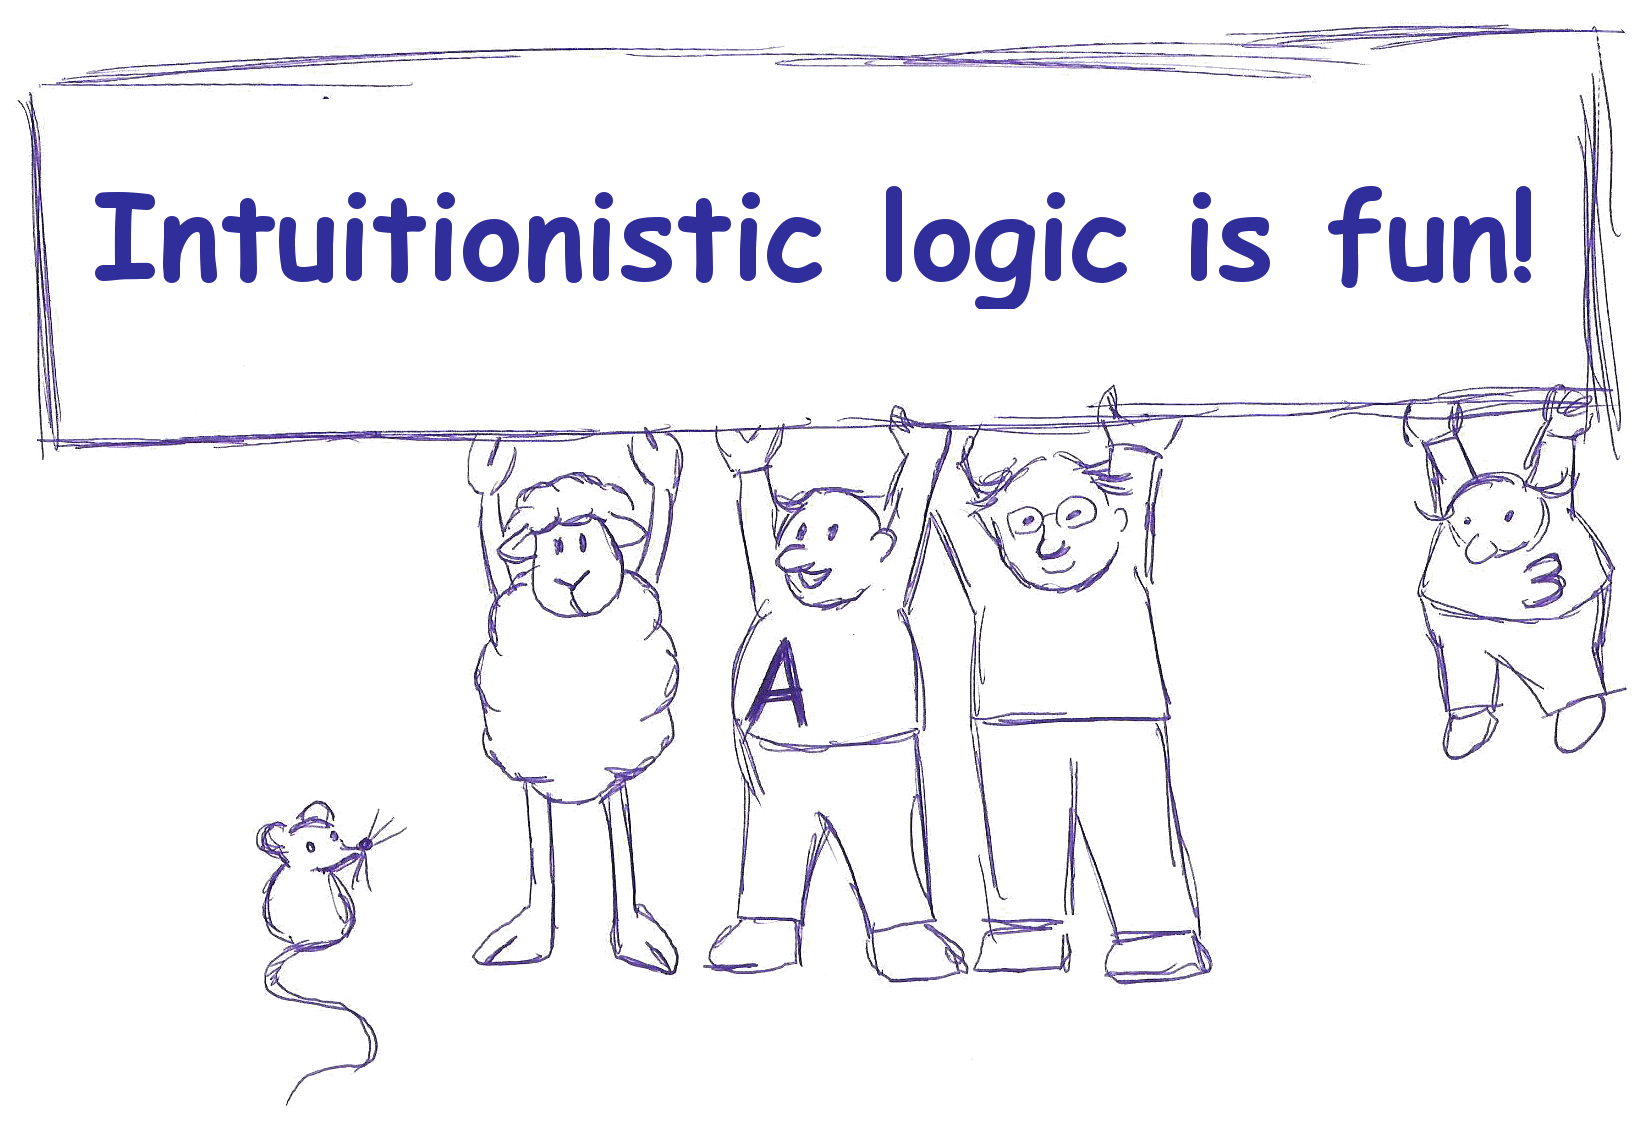
\includegraphics[height=5cm]{fun-en}}
  \only<2>{%
    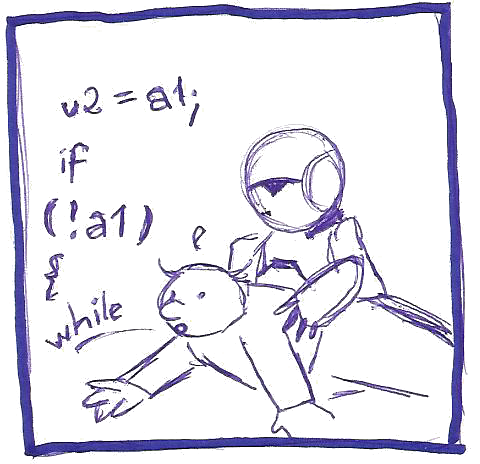
\includegraphics[height=3cm]{program-extraction}
    \hfill
    
\includegraphics[height=3cm]{constructive-maths}
    \hfill
    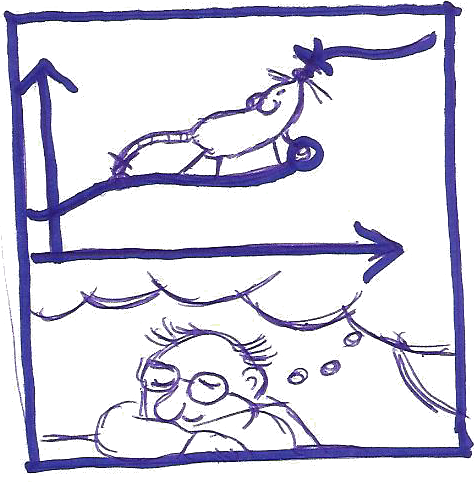
\includegraphics[height=3cm]{dream-maths}
  }
  \par
}

\note{\justifying\footnotesize
  Regarding intuitionistic logic as an elegance assisting device: In classical
  logic, we might have the habit of beginning proofs like this:

  \begin{quote}If the set~$X$ is empty, the claim holds trivially. So suppose
  that~$X$ is not empty; then consider \ldots\end{quote}
  Often it's the case that the second part of the proof applies just as fine to
  the trivial case -- if we don't fear the empty set. In these cases, the proof
  can be streamlined by skipping the case distiction.

  Intuitionistically, the case distinction is not possible without further
  hypotheses on~$X$. Therefore, by trying to make a proof intuitionistically
  acceptable, we are nudged to remove unnecessary case distictions and related
  issues.
  \par
}

\note{\justifying\footnotesize
  Here is a concrete example. Let~$f : X \to Y$ be a map and let
  \[ \renewcommand{\arraystretch}{1.3}\begin{array}{@{}rrcl@{}}
    \varphi: &\P(Y)&\longrightarrow& \P(X), \\
    & U &\longmapsto& f^{-1}[U] := \{ x \in X \,|\, f(x) \in U \}
  \end{array} \]
  be the inverse image operation. Then it's a standard exercise to show
  that~$f$ is surjective if and only if~$\varphi$ is injective.

  Can you do it, especially the ``$\Rightarrow$'' direction? There is a very
  short and elegant proof for it! But the proof which might first come to your
  mind is non-constructive and unnecessarily cumbersome:

  \begin{quote}Assume that~$f$ fails to be surjective. Then there exists~$y \in
  Y$ such that~$y$ is not an element of the image of~$f$.
  Therefore~$\varphi(\{y\}) = \emptyset = \varphi(\emptyset)$. This is a
  contradiction to the injectivity of~$\varphi$.\end{quote}

  \vfill\hfill\rotatebox{180}{\tiny\textbf{Spoiler.}
  \textcolor{gray}{We have~$\varphi(\operatorname{im} f) = X = \varphi(Y)$,
  thus~$\operatorname{im} f = Y$.}}
  \medskip
  \par
}

\note{\justifying\footnotesize
  Here is a basic example for extracting algorithms from proofs. Consider the
  statement

  \begin{quote}``There are infinitely many prime numbers.''
  \textnormal{or somewhat more explicitly,}
  ``For any finite list~$p_1,\ldots,p_n$ of prime numbers, there
  exists an additional prime number~$q$ not on that list.''\end{quote}
  The standard proof, attributed to Euclid, goes like this:

  \begin{quote}
  Consider the number~$N \defeq p_1 \cdots p_n + 1$.
  Since~$N \geq 2$, there exists some prime factor~$q$ of~$N$. (If~$N$ is
  itself prime, we can take~$q \defeq N$.)
  This prime is not equal to any~$p_i$, since the numbers~$p_i$ don't divide~$N$
  whereas~$q$ does.
  \end{quote}

  The algorithm for constructing~$q$ can be directly read off from the proof.
  Different proofs result in different algorithms; in particular, there exist
  (more complex) proofs whose algorithms produce better (smaller) witnesses.

  See the wonderful book \emph{Applied Proof Theory: Proof Interpretations and
  their Use in Mathematics} by Kohlenbach for details. Already its introduction
  is a very worthwhile reading.\par
}

\note{\justifying\footnotesize
  Tangentially, observe that the stated constructive version of Euclid's proof
  is less prone to misunderstandings than its well-known counterpart which uses
  proof by contradiction:

  \begin{quote}Assume that there are only a finite number of
  primes,~$p_1,\ldots,p_n$. Then consider~$N \defeq p_1 \cdots p_n +
  1$. This number is either prime or composite. Since no prime number
  divides~$N$ (by assumption the only primes are the~$p_i$ and these don't
  divide~$N$), it cannot be composite. Therefore~$N$ is prime. Since~$N$
  doesn't equal any of the~$p_i$, this is a contradiction.
  \end{quote}

  From this proof one might think that for primes~$p_1,\ldots,p_n$ the
  number~$N \defeq p_1 \cdots p_n + 1$ is always prime. But this only holds in
  a counterfactual world where there are only finitely many primes. In fact,
  the number
  \[ N \defeq 2 \cdot 3 \cdot 5 \cdot 7 \cdot 11 \cdot 13 + 1 = 59 \cdot 509 \]
  is composite. A shorter example is
  \[ N \defeq 2 \cdot 7 + 1 = 3 \cdot 5. \]
}

\frame{\frametitle{Topos power}
  \centering

  \begin{minipage}{0.65\textwidth}
    \begin{exampleblock}{}
      \justifying
      Any finitely generated vector space does \emph{not not} possess a basis.
    \end{exampleblock}
  \end{minipage}
  \medskip

  \scalebox{3}{$\Downarrow$}

  \begin{minipage}{0.65\textwidth}
    \begin{exampleblock}{}
      \justifying
      Any sheaf of modules of finite type on a \mbox{reduced} scheme is locally free on a dense
      open subset.
    \end{exampleblock}
  \end{minipage}
  \par
}

\note{\justifying\footnotesize
  Toposes are certain kinds of categories, thought of as \emph{mathematical
  universes}. The usual topos in which we do mathematics in is the category of
  sets and maps between sets, but there are many others:
  \begin{itemize}
  \item In the \emph{effective topos}, any map is computable.
  \item In the \emph{sheaf topos} of a topological space~$X$ the objects and
  morphisms depend on our position in~$X$.
  \end{itemize}
  A metatheorem states that \emph{intuitionistically provable statements hold
  in any topos}. This greatly expands the scope of an intuitionistic theorem.

  A side project of mine is to recognize the basic concepts and statements of
  algebraic geometry as topos-theoretic interpretations of simple concepts and
  statements of ordinary first-year linear algebra. See
  \url{https://github.com/iblech/internal-methods} for expository notes on this
  topic (directed at geometers). The example of the slide is taken from these
  notes. The simple statement about vector spaces \emph{automatically implies}
  the more complicated statement about sheaves.
  \par
}

\frame{\frametitle{Dream mathematics}
  \centering

  \begin{minipage}{0.85\textwidth}
    \begin{block}{\centering Synthetic differential geometry}
      \justifying
      Any map~$\RR \to \RR$ is smooth. There are in\-fi\-ni\-te\-si\-mal
      numbers~$\varepsilon$ such that~$\varepsilon^2 = 0$ and~$\varepsilon \neq 0$.
    \end{block}
  \end{minipage}

  \begin{minipage}{0.85\textwidth}
    \begin{block}{\centering Synthetic domain theory}
      \justifying
      For any set~$X$ there exists a map
      \vspace*{-0.9em}
      \[ \fix : (X \to X) \to X \]
      \vspace*{-2.1em}

      such that
      $f(\fix(f)) = \fix(f)$ for any~$f : X \to X$.
    \end{block}
  \end{minipage}

  \begin{minipage}{0.85\textwidth}
    \begin{block}{\centering Synthetic computability theory}
      \justifying
      There are only countably many subsets of~$\NN$.
    \end{block}
  \end{minipage}

  \par
}

\note{\justifying\footnotesize
  Dream mathematics is working with dream axioms -- axioms which are
  classically false, but very convenient:
  \begin{itemize}\justifying
  \item If you adopt synthetic differential geometry, you can do calculus like
  300 hundred years ago, by manipulating infinitesimals.
  See \styledhref{http://math.andrej.com/2008/08/13/intuitionistic-mathematics-for-physics/}{a blog post by Andrej Bauer}.
  \item If you adopt synthetic domain theory, you can use the ordinary
  mathematical notions of sets and maps to give semantics to programming
  languages. See
  \styledhref{http://homepages.inf.ed.ac.uk/als/Talks/lfps04.pdf}{slides of a talk by
  Alex Simpson} and
  \styledhref{https://www.dpmms.cam.ac.uk/~martin/Research/Oldpapers/synthetic91.pdf}{a
  paper by Hyland}.
  \item If you adopt synthetic computability theory, you can use the ordinary
  notions of sets and maps to really talk about enumerable sets and computable
  maps. You can drop any of the usual adjectives like ``effectively'' or
  ``enumerable''. See \styledhref{http://math.andrej.com/data/synthetic.pdf}{a paper
  by Andrej Bauer}.
  \end{itemize}

  All of these dream axioms can be made to work: By dropping the law of
  excluded middle. More precisely, there are alternate toposes in which the law
  of excluded middle does not hold but the given dream axiom does. Also there
  are metatheorems which guaranteed that results obtained in the dream universe
  also hold in the the usual universe.

  \emph{Warning.} For space reasons, the axioms are not presented faithfully on
  the previous slide. Check the references for precise formulations.
  \par
}

\section{The double-negation translation}

\subsection{The doubly-negated law of excluded middle}

\frame{\frametitle{The doubly-negated LEM}
  \centering
  Even intuitionistically ``$\neg\neg(A \,\vee\, \neg A)$'' holds.
  \par

  \begin{minipage}{0.90\textwidth}
    \begin{exampleblock}{}
      \justifying
      \textbf{Proof.} Assume~$\neg(A \vee \neg A)$, we want to show~$\bot$. \\[0.3em]
      If~$A$, then~$A \vee \neg A$, thus~$\bot$. Therefore~$\neg A$. \\[0.3em]
      Since~$\neg A$, we have $A \vee \neg A$, thus~$\bot$.
    \end{exampleblock}
  \end{minipage}
  \par
}

\subsection{The fundamental result}

\newcommand{\inegneg}{{\usebeamercolor[fg]{item}{\boldsymbol{\neg\neg}}}}
\newcommand{\gnegneg}[1]{\textcolor{gray}{\boldsymbol{\neg\neg}(}#1\textcolor{gray}{)}}

\frame{\frametitle{The $\boldsymbol{\neg\neg}$-translation}
  \vspace*{-2em}
  \begin{align*}
    A^\Box &\defeqv \inegneg A \text{ for atomic formulas~$A$} \\
    (A \wedge B)^\Box &\defeqv \gnegneg{A^\Box \wedge B^\Box} \\
    (A \vee B)^\Box &\defeqv \inegneg(A^\Box \vee B^\Box) \\
    (A \Rightarrow B)^\Box &\defeqv \gnegneg{A^\Box \Rightarrow B^\Box} \\
    (\forall x{:}X\_ A(x))^\Box &\defeqv \gnegneg{\forall x{:}X\_ A^\Box(x)} \\
    (\exists x{:}X\_ A(x))^\Box &\defeqv \inegneg(\exists x{:}X\_ A^\Box(x))
  \end{align*}

  \hil{Theorem.} $A$ classically $\Longleftrightarrow$ $A^\Box$ intuitionistically.
}

\note{\justifying\footnotesize
  The gray \textcolor{gray}{$\neg\neg$}'s can be omitted: One can prove by
  structural induction that translating with those double negations yields
  logically equivalent formulas as translating without those.

  The blue $\inegneg$'s in contrast are crucial.

  One could say that the only difference between intuitionistic logic and
  classical logic is in the meaning of disjunction and existential
  quantification.

  If~$A$ does not contain~``$\Rightarrow$'' and~``$\forall$'', then~$A^\Box
  \Leftrightarrow \not\not A$. Such formulas are also called \emph{geometric},
  because their truth value is preserved by so-called \emph{geometric functors}
  in topos theory. In general, there is no implicational relation
  between~$A^\Box$ and~$\not\not A$.
  \par
}

\note{\justifying\footnotesize
  Note that~$\bot^\Box \equiv \neg\neg\bot \Leftrightarrow \bot$.

  \textbf{Corollary.} Peano arithmetic and Heyting arithmetic are equiconsistent.
  (Recall that Heyting arithmetic is the same as Peano arithmetic, only with
  intuitionistic instead of classical logic.)

  \textbf{Proof.} It is clear that inconsistency of Heyting arithmetic implies
  inconsistency of Peano arithmetic.

  For the converse direction, write~$\mathrm{Ax}$ for the axioms of Peano
  arithmetic, thought of as a single formula by conjuction. If Peano arithmetic
  proves~$\bot$, that is if~$\mathrm{Ax} \Rightarrow \bot$ classically, then by
  the theorem~$\mathrm{Ax}^\Box \Rightarrow \bot^\Box$ intuitionistically. By
  inspection~$\mathrm{Ax} \Rightarrow \mathrm{Ax}^\Box$ intuitionistically.
  Therefore~$\mathrm{Ax} \Rightarrow \bot$ intuitionistically.
  \par
}

\subsection{Game-theoretical interpretation}

\note{
  \centering
  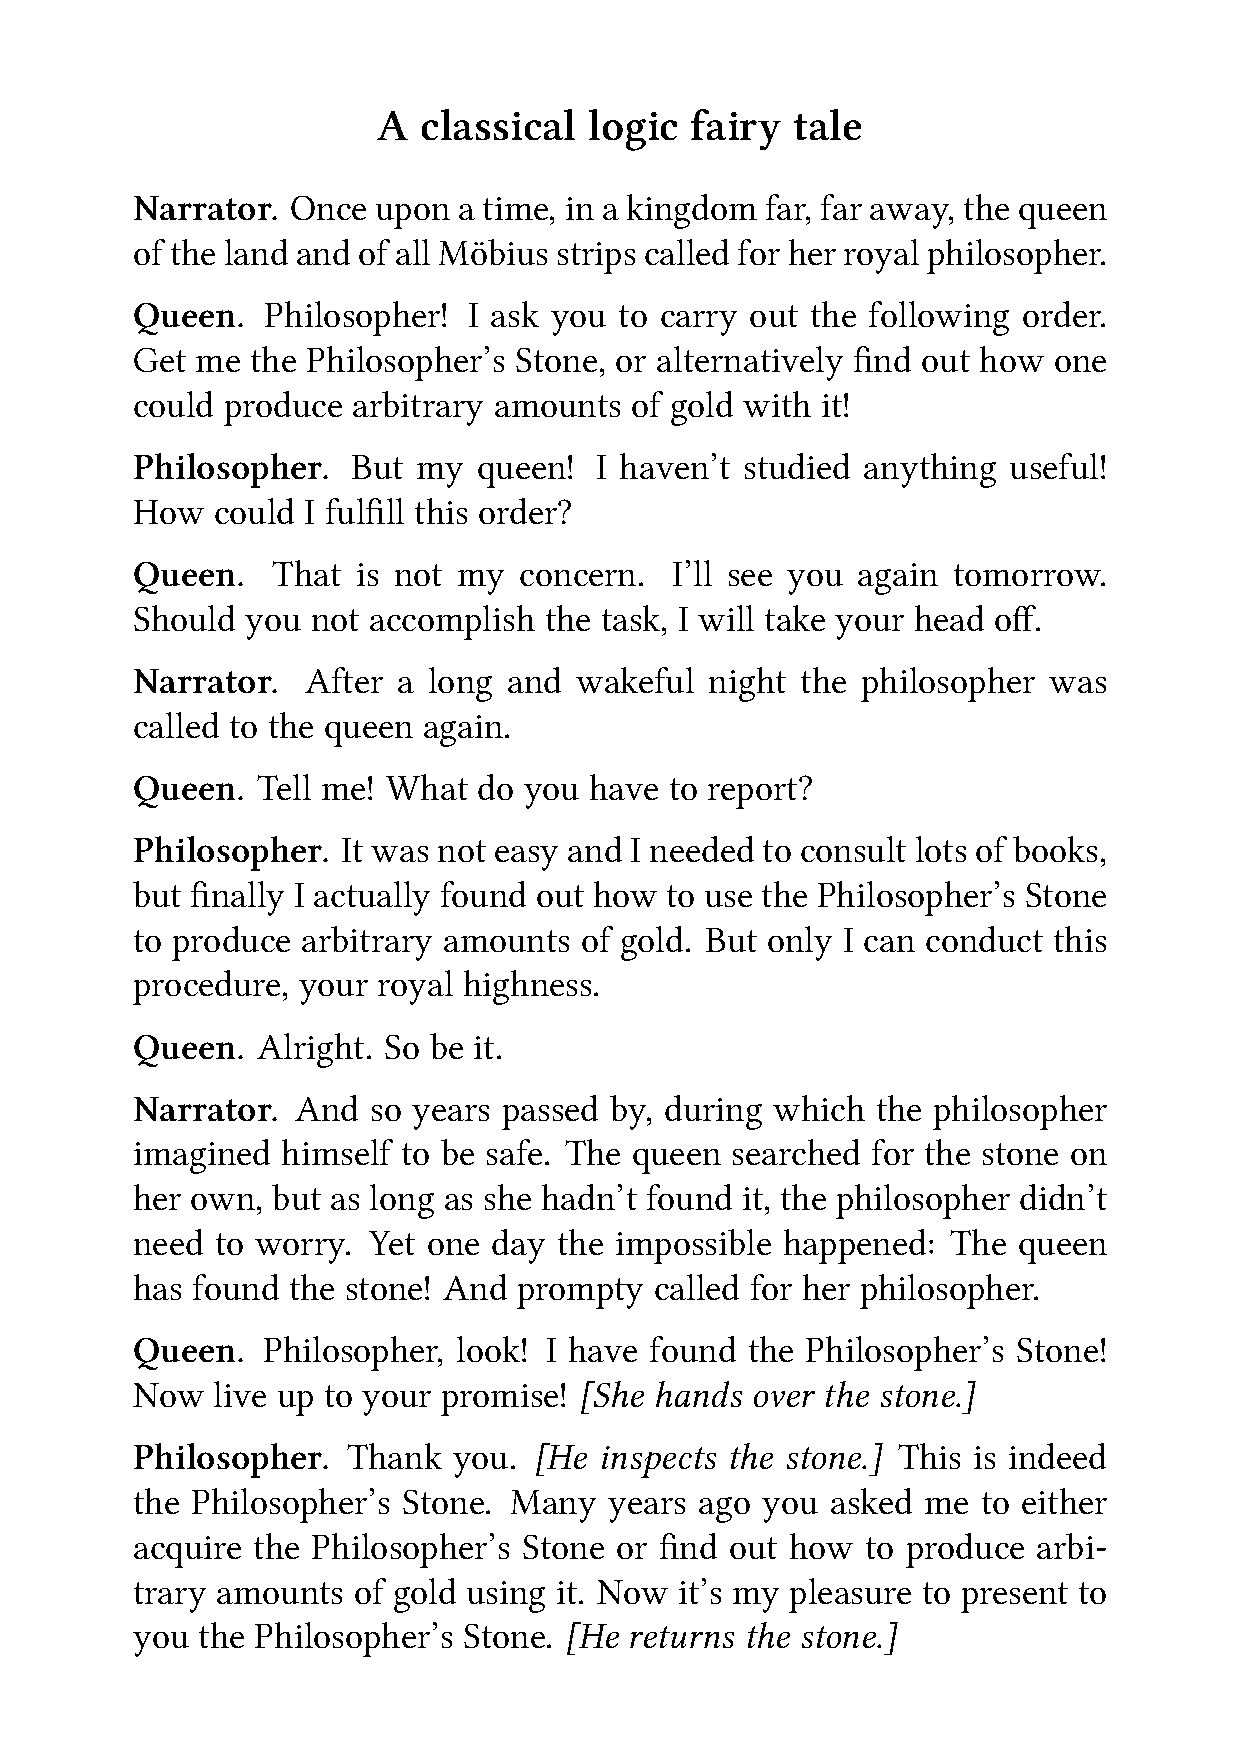
\includegraphics[height=\textheight]{philosophers-stone}
  \par
}

\frame{\frametitle{A classical logic fairy tale}
  % http://www.geekalerts.com/u/Collectible-Harry-Potter-Sorcerers-Stone1.jpg
  {\centering 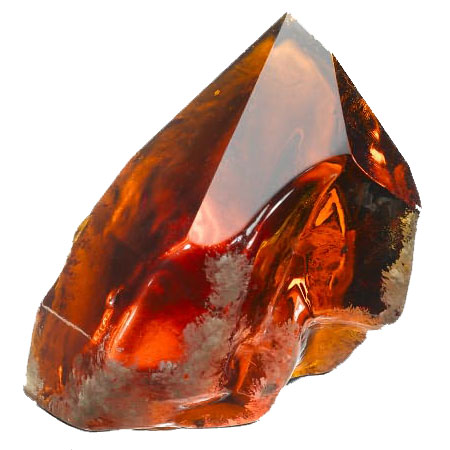
\includegraphics[scale=0.25]{philosophers-stone.jpeg}\par}
  \pause

  \begin{changemargin}{-0.9em}{-0.9em}
  $A$ intuitionistically \tabto{3.93cm}$\Longleftrightarrow$
  we can defend~$A$ in any dialog.
  \bigskip

  \tabto{1.3cm}$A$ classically \tabto{3.93cm}$\Longleftrightarrow$
  we can defend~$A^\Box$ in any dialog.
  \pause

  \tabto{3.93cm}$\Longleftrightarrow$
  we can defend~$A$ in any dialog \\
  \tabto{3.93cm}$\phantom{\Longleftrightarrow}$ with jumps back in time allowed.
  \end{changemargin}
}

\note{\justifying\footnotesize
  Recall the usual dialog metaphor for proofs:

  \begin{quote}
    \textbf{Alice.} I claim that~$\forall x:X\_ A(x) \Rightarrow B(x)$.

    \textbf{Eve.} Really? Take this particular~$x_0:X$!

    \textbf{Alice.} Sure. Then I claim that~$A(x_0) \Rightarrow B(x_0)$.

    \textbf{Eve.} My~$x_0$ satisfies~$A(x_0)$, see? \ldots

    \textbf{Alice.} Right. And from this I'm able to show~$B(x_0)$: \ldots
  \end{quote}

  This metaphor can be formalized. Then it's a theorem that a statment~$A$
  holds intuitionistically if and only if the proponent has a winning strategy
  for dialogs about~$A$. See the survey article by Helger Rückert in
  \emph{Essays on Non-Classical Logic} for details.

  Reading~``$A$'' for~``Philosopher's Stone'' and~``$A \Rightarrow \bot$'' for
  ``using the Philosopher's Stone to produce arbitrary amounts of gold'', the
  classical logic fairy tale gives a proof of the law of excluded middle -- in
  dialog form, with time jumps.
  See \styledhref{http://blog.ezyang.com/2013/04/a-classical-logic-fairy-tale/}{this
  blog post by Edward Yang} for a different rendition of the tale and for
  references.

  It is not a coincidence that the tale feels ``continuation-y''.
  \par
}

\section{Continuations}

\subsection{The Curry--Howard correspondence}

\frame{\frametitle{Curry--Howard correspondence}
  \centering
  \setlength{\extrarowheight}{0.3em}
  \begin{tabular}{r@{\quad}l}
    \hil{logic} & \hil{programming} \\
    formula $A$ & type $A$ \\
    intuitionistic proof $p:A$ & term $p:A$ \\
    conjuction $A \wedge B$ & product type $(A,B)$ \\
    disjunction $A \vee B$ & sum type \textsf{Either} $A$ $B$ \\
    implication $A \Rightarrow B$ & function type $A \to B$ \pause \\
    \hil{$\inegneg$-translation} & \hil{CPS transformation} \pause \\
    \only<3>{$\neg\neg A$ & ?? \\} \pause
    \only<4>{$(A \Rightarrow \bot) \Rightarrow \bot$ & ?? \\} \pause
    $(A \Rightarrow \bot) \Rightarrow \bot$ & $(A \to r) \to r$
  \end{tabular}

  \par
}

\note{\justifying\footnotesize
  On the previous slide $r$ should denote the void type (having no
  inhabitants). But this is a bit boring; we can also use any type for~$r$ and
  employ a variant of the double-negation translation: One where we don't
  use~$\neg\neg$, but~$\neg_r \neg_r$, where~$\neg_r$ is defined as~$\neg_r A
  \defeq (A \Rightarrow r)$. For this variant, it still holds that we can
  transform classical proofs of~$A$ into intuitionistic proofs of~$A^{\Box_r}$.

  To see that the double-negation translation corresponds to the CPS
  transformation, simply note that the type~$(a \rightarrow r) \rightarrow r$ is also
  known under the name~\textsf{Cont}~$r$~$a$.

  Different but logically equivalent versions of the double-negation
  translation yield different variants of the CPS transformation (call by name,
  call by value, \ldots).
  \par
}

\subsection{Computational content of classical proofs}

\begin{frame}[fragile]\frametitle{Computational content of classical proofs}
  \begin{changemargin}{-0.5em}{-0.5em}
  \begin{minted}{haskell}
type Cont r a = ((a -> r) -> r)

-- Decide an arbitrary statement a.
lem :: Cont r (Either a (a -> Cont r b))
lem k = k $ Right $ \x -> (\k' -> k (Left x))

-- Calculate the minimum of an infinite list
-- of natural numbers.
min :: [Nat] -> Cont r (Int, Int -> Cont r ())
min xs = ...
  \end{minted}
  \end{changemargin}
\end{frame}

\note{\justifying\footnotesize
  To decide an arbitrary statement~$A$, we proceed as follows. When asked
  whether~$A$ or~$\neg A$ holds, we bluff and immediately claim that~$\neg A$
  holds. Since~$\neg A$ is defined as~$(A \Rightarrow \bot)$, \emph{our
  opponent has to work in order to rebut our claim}. As soon as our opponent
  presents evidence for~$A$, we rewind time and make it look as if we always
  claimed that~$A$ holds from the start.

  Similarly, to find the minimum of an infinite list~$(x_n)_n$ of natural numbers, we
  simply claim the first number~$x_0$ of the list is the minimum. This might actually
  be true. Should our opponent later present a smaller element~$x_i$, we rewind time
  (take a previously-stored continuation) and claim that~$x_i$ is the minimum.
  This process of refining our initial guess will terminate after at most~$x_0$
  many time jumps.
  \par
}

\note{
  \begin{center}\large\textbf{Food for thought}\end{center}

  \classicalcontent
}

\note{\justifying\footnotesize
  Here is a practical example from algorithmic number theory for the use of the
  ``computational law of excluded middle''. Let~$x$ be an algebraic number,
  that is a complex number which is a zero of a normed polynomial~$f(X) \in \QQ[X]$.
  Consider the field extension~$\QQ(x)$ of~$\QQ$ generated by~$x$; this field
  contains the rational numbers, the number~$x$, and every number which can be
  obtained from these by addition, subtraction, multiplication, and division.

  We want to describe an algorithm for computing the inverse of a nonzero
  element in~$\QQ(x)$ and expressing this inverse as a polynomial in~$x$. In
  principle, this can be done as follows.

  Factor~$f(X)$ into irreducible polynomials. One of the factors, say~$g(X)$,
  will be zero at~$x$. This factor is called the \emph{minimal polynomial}
  of~$x$ and general theory tells us that~$\QQ(x) \cong \QQ[X]/(g(X))$; so
  working in~$\QQ(x)$ is the same as working in the polynomial ring~$\QQ[X]$
  modulo~$g(X)$. Since the extended Euclidean algorithm provides an efficient
  method for finding modular inverses, it looks like we are done.

  However, factoring~$f(X)$ into irreducible polynomials is computationally
  expensive. Is there a way to avoid that?
  \par
}

\note{\justifying\footnotesize
  Yes! Let~$[h(X)] \in \QQ[X]/(f(X))$. We want to compute a modular inverse
  to~$h(x)$ in~$\QQ(x)$. Note that since~$f(X)$ might not be irreducible, the
  ring~$\QQ[X]/(f(X))$ might not be a field (any factor of~$f(X)$ is a zero
  divisor in this ring). Nevertheless, we can use the extended Euclidean
  algorithm to compute the (monic) greatest common divisor~$d(X)$ of~$f(X)$ and~$h(X)$
  and a \emph{Bézout representation}
  \[ d(X) = a(X) f(X) + b(X) h(X). \]
  Three cases can occur:
  \begin{enumerate}\justifying\scriptsize
  \item $d(X) = 1$. Then the equation shows that~$b(X)$ is inverse to~$h(X)$
  modulo~$f(X)$ (and therefore, \emph{a fortiori}, modulo the
  inaccessible~$g(X)$). In particular,~$b(x)$ is inverse to~$h(x)$ in~$\QQ(x)$.
  \item $d(X) = f(X)$. Then the equation shows that~$h(X)$ is a multiple
  of~$f(X)$ and therefore~$h(x)$ is zero. In this case we don't need (and
  can't) compute an inverse.
  \item Else~$d(X)$ is a nontrivial factor of~$f(X)$. At least one of the
  polynomials~$d(X)$ and~$f(X)/d(X)$ still has~$x$ as a zero. Call this
  polynomial~$\tilde f(X)$. Then restart the calculation using~$\tilde
  f(X)$ instead of~$f(X)$.
  \end{enumerate}
  In this way we can work in~$\QQ[X]/(g(X))$ without having to explicitly
  compute~$g(X)$. ``Leaving the continuation monad'' is not a problem, since
  inverses modulo~$f(X)$ or~$\tilde f(X)$ or~$\tilde{\tilde f}(X)$
  are also inverses modulo the proper~$g(X)$.
  \par
}

\section{Outlook}

\frame{\frametitle{Outlook}
  \begin{itemize}
    \item CPS transformation $=$ Yoneda embedding
    \item Geometrical interpretation:
    \[ \Sh(X) \models A^\Box \quad\Longleftrightarrow\quad
    \Sh(X_{\neg\neg}) \models A \]
    \item Generalize from~$\neg\neg$ to arbitrary \hil{modal
    operators} (monads): Relevant axioms are
    \begin{enumerate}
      \item $A \Rightarrow \Box A$
      \item $\Box\Box A \Rightarrow \Box A$
      \item $\Box(A \wedge B) \Leftrightarrow \Box A \wedge \Box B$
    \end{enumerate}
  \end{itemize}
  \pause

  \centering
  \href{https://github.com/iblech/talk-constructive-mathematics}{
\includegraphics[height=2em]{github}\textsf{/iblech/talk-constructive-mathematics}}
  \par
}

\note{\justifying\footnotesize
  Recommended reading:
  \begin{itemize}
    \item \styledhref{http://okmij.org/ftp/Computation/lem.html}{Oleg Kiselyov on the law of excluded middle}.
    \item Chetan Murthy's PhD thesis
    \styledhref{http://ecommons.library.cornell.edu/bitstream/1813/6991/1/90-1151.pdf}{Extracting
    Constructive Content from Classical Proofs}.
    \item The \styledhref{http://math.andrej.com}{blog of Andrej Bauer},
    especially the posts tagged \texttt{constructive-math}.
  \end{itemize}
}

\end{document}

Start with the Spiked Math comic, of course.

1. Constructive mathematics
   * LEM
   * (Informal) BKH interpretation
   * Applications
     (in "note" slides state that the word "contradiction" is not forbidden per se)

2. The double-negation translation
   * Proof of neg neg (phi v neg phi)
   * The translation and the fundamental result
   * Game-theoretical interpretation

3. Relation to continuations
   * Curry--Howard correspondence
   * negneg-translation = CPS transformation
   * Computational content of classical proofs

4. Outlook
   * CPS transformation = Yoneda embedding
   * Box-translation for arbitrary modal operators Box
   * negneg-sheafification?


* http://www.reddit.com/r/math/comments/1fp3q9/how_is_the_double_negation_translation_similar_to/
* http://stackoverflow.com/questions/2969140/what-are-the-most-interesting-equivalences-arising-from-the-curry-howard-isomorp/2969800#2969800
* http://okmij.org/ftp/Computation/lem.html

* State that (neg neg A ==> A) is like catching an exception.

* Also state Friedman's Trick? And applications? For instance, halting of
  Turing machines.

* According to many-happy-returns.ps, logical contents of delimited
  continuations are explored by Kamenaya.

* Murthy's PhD thesis! Give him due credit.
  (Murthy was a student of Robert Constable (Cornell), who in turn was a
  student of Kleene.)

* Cite Helger Rückert in /Essays on Non-Classical Logic/

* Case study: Minimum of a set of natural numbers.
  In which sense do we know that the algorithm terminates?

* Axiom of choice.

http://math.andrej.com/wp-content/uploads/2014/03/real-world-realizability.pdf
